\documentclass[conference]{IEEEtran}
\newtheorem{definition}{Definition}
\usepackage{paralist}
\usepackage{url}
\usepackage{graphicx}
\usepackage{amsmath,amssymb}
\usepackage{listings}
\usepackage{tikz}
\usepackage{color}
\usetikzlibrary{trees}


\def\collapse#1{\textcolor{blue}{\ensuremath{\mathord{\blacktriangleleft}
\mathord{#1}
\mathord{\blacktriangleright}}}}

% \DeclareUnicodeCharacter{B1}{\pm}
%% LANGUAGE      Markup definitions
\def\lstxml{
  \lstset{language=XML,
    basicstyle=\scriptsize,
    keywordstyle=\bfseries\ttfamily,
    identifierstyle=\ttfamily, 
    % commentstyle=\color{Brown},
    stringstyle=\ttfamily,
    showstringspaces=false,
    columns=[l]flexible, %% , basewidth={0.5em,0.4em}
    escapeinside={(@*}{*@)},
    deletekeywords={type,id}, % does not work!
    otherkeywords={encoding,
      mrow,math,mfrac,mi,msqrt,mo,mn,span,nobr,img,msup,maction,mtext}
  }
}
\def\lsthtml{
\lstset{language=html,
    basicstyle=\scriptsize,
    keywordstyle=\bfseries\ttfamily,
    showstringspaces=false,
    % otherkeywords={mfenced, open, close, separators, mrow, mi, mo, mn, math, 
    %   msup, role, parent, children, added}
}
}

\def\latex{\LaTeX}


\begin{document}

\title{Employing Semantic Analysis for Enhanced Accessibility Features in
  MathJax}

\author{\IEEEauthorblockN{Davide Cervone}
  \IEEEauthorblockA{MathJax Consortium\\
    Union College, NY\\
    Email: \url{dpvc@union.edu}\\
    %% URL: \url{www.mathjax.org}
  }
  \and
  \IEEEauthorblockN{Peter Krautzberger}
  \IEEEauthorblockA{MathJax Consortium\\
    krautzource UG\\
    Email: \url{peter.krautzberger@mathjax.org}\\[.2cm]
    URL: \url{www.mathjax.org}}
  \and  \IEEEauthorblockN{Volker Sorge}
  \IEEEauthorblockA{MathJax Consortium\\
    University of Birmingham, UK\\
    Email: \url{V.Sorge@cs.bham.ac.uk}\\
    %% URL: \url{www.cs.bham.ac.uk/~vxs}
  }
  %% Thanks does not seem to work.
  \thanks{This work was partially supported by the Alfred P. Sloan Foundation.}
}


\maketitle

\begin{abstract}
  Recent changes in the landscape for assistive technology solutions for
  Mathematics on the web have prompted the development of MathJax into a single
  rendering and accessibility solution. We present our current efforts that
  depend on a novel semantic interpretation of Presentation MathML
  expressions. This allows us to introduce a new notion of responsive equations,
  on which we build advanced accessibility features with improved reflow of
  content, selective highlighting, and dynamic speech text generation, as well as
  an innovative interaction technique based on abstracting and intelligently
  summarising sub-expressions.
\end{abstract}
\IEEEpeerreviewmaketitle

\begin{IEEEkeywords}
  STEM Accessibility, Mathematics, MathJax
\end{IEEEkeywords}

\section{Introduction}

The text-to-speech translation of mathematical expressions has always been a
challenging problem and is one major obstacle for fully inclusive
education. Consequently, a number of software solutions have been researched
over the years (see~\cite{karshmer2007mathematics} for an overview). As web
delivery grows, web-accessibility for mathematics is more important than ever.

Although formulas can be represented in their own specialised markup language
(MathML~\cite{MathML3}, part of HTML5~\cite{HTML5}), only Firefox and Safari
partially support it. Besides low market shares \cite{browser_stats} they fall
short in functionality such as basic elements (e.g., \texttt{maction} on Safari)
or APIs (e.g., GlobalEventHandler on Firefox). Thus support for displaying
formulas represented in MathML on web pages is sketchy. Rendering tools like
MathJax \cite{MathJax2.5} can provide high-quality cross-browser rendering but
have to decouple accessible rendering from visual rendering by providing raw
MathML visually hidden.

To overcome this problem, MathJax is developing a complete accessibility 
solution that works in all browsers providing improved reflow, navigation, 
collapse and expansion, selective highlighting, and dynamic speech-text 
generation. 

Since Presentation MathML is not expressive enough to provide accessible
rendering, we developed heuristics for semantically enriching Presentation
MathML and, by extension, any other MathJax-compatible input such as {\LaTeX} 
and AsciiMath. These heuristics use MathML's tree structure to build a tightly
related semantic tree that is injected into the presentation elements. This
allows us to easily expose the identified semantic structure in the DOM, and
this structure is used in turn to generate alternate representations such as
speech text, and when combined with the underlying Presentation MathML tree,
responsive rendering and exploration interfaces.

\section{Math accessibility on the Web}
\label{sec:math}

Before 2012, math accessibility on the web was synonymous with
MathPlayer~\cite{soiffer2005mathplayer} on Internet Explorer. With IE11
deprecating plugins like MathPlayer, and ChromeVox~\cite{Sorge14} and
VoiceOver~\cite{voiceover} adding some MathML support, the landscape grew more
complex. Unfortunately, the core problem for web-based math accessibility has
not changed: browsers offer very limited MathML support. Consequently
mathematics on the web comes in the following flavors:
\begin{inparaenum}
\item \textbf{Pure MathML markup} relying on the user to view the page with one
  of the few MathML-capable browsers.
\item \textbf{Pre-rendered binary images} to ensure correct, low-quality 
  display, at most embedding the original markup in alt-text.
\item \textbf{Rendered with MathJax} so the web page author ensures   
  mathematical content is rendered independent of the browser.
\item In a more recent trend, \textbf{pre-rendered markup} (usually with MathJax
  running on NodeJS) ensures correct display by including HTML (with CSS) or SVG
  in the web page.
\end{inparaenum}

\begin{figure}[b]
  \centering
\lstxml
\begin{lstlisting}[language=XML,basicstyle=\small]
        <math>
          <mi>a</mi>
          <msup>
            <mi>x</mi>
            <mn>2</mn>
          </msup>
          <mo>+</mo>
          <mi>b</mi>
          <mi>x</mi>
          <mo>+</mo>
          <mi>c</mi>
          <mo>=</mo>
          <mn>0</mn>
        </math>
\end{lstlisting}
\caption{MathML representation of the quadratic equation.}
\label{fig:syntactic-tree}
\end{figure}
\begin{figure*}[t!]
  \begin{center}
    \leavevmode
    \lsthtml
    \lstinputlisting{mathjax.xml}
    \caption{Abbreviated MathJax HTML representation of the quadratic formula.}
    \label{fig:mathjax}
  \end{center}
\end{figure*}


Hence rendering solutions like MathJax remain critical for authors and
users, becoming the de facto standard for Mathematics rendering on the web in
the past five years. MathJax covers 85\% of the MathML3 test suite and provides
input processors for commonly used languages such as {\TeX/\LaTeX} and
AsciiMath. It is used by most major scientific and educational publishers as
well as large platforms such as StackExchange, edX, Quora, and
Wikipedia. MathJax's free CDN service sees over 4.5 million unique daily
visitors.

It is difficult for MathJax to provide fully accessible output, however, as the
only web standard for math accessibility is indeed MathML. ARIA, for example,
does not provide roles for exposing mathematical information beyond the global
math role.  But since MathML can not be rendered natively in many browsers,
MathJax has to carefully separate accessible MathML from the visual output.  To
illustrate this point, consider the simple example of the quadratic equation
\({ax^2+bx+c=0}\).
Its MathML expression is given in Fig.~\ref{fig:syntactic-tree}. While this can
be exposed to assistive technology (AT), e.g., to VoiceOver or ChromeVox
directly and to other AT vendors via the new MathPlayer library, it must be
hidden from the browsers themselves, as they usually cannot render it. On the other hand,
MathJax's actual visual rendering (given in HTML/CSS format in
Fig.~\ref{fig:mathjax}), must be hidden from the AT to avoid it producing
gibberish.

Since most mathematics on the web is rendered by MathJax, this provides a unique
opportunity to combine accessibility features with its visual rendering.
MathJax already provides basic AT features such as magnification and global
scaling (see section \ref{sec:responsive-equations}).  Both can negatively affect
users with learning disabilities, in particular those who benefit from a less
overloaded layout. Highlighting suffers from similar limitations as one can at
best highlight the underlying MathML tree, which may not necessarily group
sub-expressions semantically.

The speech translation of mathematics poses unique difficulties that make it a
more challenging task than the aural rendering of text. Difficulties
include:
the wide spectrum of symbols,
use and importance of punctuation as well as white space, and
complex two-dimensional math layout.
While there exist rule sets for
translating mathematical expressions into speech (e.g.,
MathSpeak~\cite{MathSpeak}) they usually require some interpretation of the
mathematics that goes beyond what Presentation MathML alone can offer.  We
therefore have designed a novel semantic enrichment method for MathML that
allows the implementation of advanced accessibility features in
MathJax.

\section{Semantic Enrichment}
\label{sec:semantic-enrichment}

Our main improvements for accessible rendering of mathematics rely on a semantic
enrichment of presentation MathML elements. This is based on a heuristic
analysis of the syntactic structure of MathML elements as a semantic tree, and
aims to stay faithful to the given notation while avoiding false semantic
interpretations as much as possible. Although this leads to a more shallow
interpretation than a full-blown semantic markup language like Content
MathML~\cite{MathML3}, it has the advantage that it retains effectively all the
components of the original expression. While in Content MathML, symbols like
parentheses are omitted and entire expressions are replaced by their semantic
counterparts, we aim to retain these as they are important for both visual and
aural rendering.  Moreover, it allows us to combine the semantic interpretation
with the presentation form by embedding it via HTML attributes, with limited,
conservative remodelling of the original MathML expression. This allows the
presentation element tree to provide a different view of the MathML expression
without having to maintain a separate structure in parallel, which would be
necessary if exploiting MathML's \texttt{semantics} tag.

While there exist methods for translating mathematical syntax into Content
MathML, they either restrict the mathematics to what a particular computer
algebra system can handle~\cite{Maple,Mathematica} or are based solely on
{\LaTeX} interpretation~\cite{miller2010latexml, mooresemantic, SnuggleTeX}.
Our semantic tree, on the other hand, is built to handle any mathematical
notation found in arbitrary web documents.  We first briefly sketch the major
ideas of the semantic-tree generation --- an extension of the heuristics
implemented in the screen reader ChromeVox~\cite{Sorge14} --- and then describe
how its information is integrated into existing MathML structures.

\subsection{Semantic Tree}
\label{sec:semantic-tree}

The main problem for semantic enrichment of Presentation MathML is to transform
its flat structure into one that correctly determines the scope of operators,
relations, etc.  Our approach aims to represent a formula in a semantic tree
structure akin to a term tree. The semantic tree is assembled bottom-up, where
we first classify the single components of an expression, giving each an
immutable type and a mutable role. The former aims to capture the basic nature
of the symbol, while the latter is used to describe the role of a symbol in the
context of the formula. For example, $f$, which has the type of ``identifier'', gets
a default role of ``Latin letter'' assigned while no additional information is
known. Once more knowledge of its semantic meaning is available, its role is
refined. For example, in the expression $f(x)$ it would get the role of a
``function'', while its role remains unchanged in $f + g$.

A central heuristic then builds term trees from flat structures by promoting
relations and defining operator precedence orders as well as determining
properly delimited structures.  As an example of this heuristic we observe how
the quadratic equation $ax^2 + bx + c = 0$ is rewritten from Presentation
MathML (Fig.~\ref{fig:syntactic-tree}) into its semantic
interpretation (Fig.~\ref{fig:semantic-tree}).

\begin{figure}[t]
  \centering
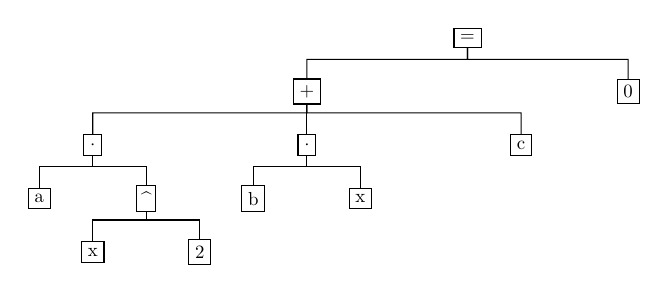
\begin{tikzpicture}[scale=.68, transform shape,
  level 1/.style={sibling distance=4cm,level distance=.8cm}
  ]
  \node[draw] {=}
  [grow via three points={one child at (0,-1.25) and two children at
(-3,-1) and (3,-1)}, edge from parent fork down]
  child {node[draw] {+}[grow via three points={one child at (0,-1) and
two children at (-2,-1) and (2,-1)}, edge from parent fork down]
  child {node[draw] {$\cdot$}[grow via three points={one child at
      (0,-1) and two children at (-1,-1) and (1,-1)}, edge from parent fork 
down]
    child {node[draw]{a}}
  child {node[draw] {$\,\widehat{}\,$}[grow via three points={one
      child at (0,-1) and two children at (-1,-1) and (1,-1)}, edge from parent 
fork
    down]
    child {node[draw]{x}}
    child {node[draw]{2}}}
        }
  child {node[draw] {$\cdot$}[grow via three points={one child at
      (0,-1) and two children at (-1,-1) and (1,-1)}, edge from parent fork 
down]
    child {node[draw]{b}}
    child {node[draw]{x}}
        }
  child {node[draw]{c}}
        }
  child {node[draw] {0}}
  ;
\end{tikzpicture}
  \caption{Semantic term tree for the quadratic equation.}
  \label{fig:semantic-tree}
\end{figure}

Observe that the transformation tries hard to recognise elided multiplications.
In addition, our procedure contains a number of heuristics, in particular to
\begin{inparaenum}[(1)]
 \item determine potential function applications,
 \item break up symbol sequences into elided products,
 \item recognise scope and nesting of big operators (e.g., sums, integrals),
 \item distinguish tables into matrices, vectors, and case statements,
 \item combine punctuated expressions and determine the meaning of ellipses.
\end{inparaenum}

Technically the tree is constructed by analysing MathML elements, interpreting
their type, role, and font, and turning them into semantic nodes with parent
pointer and a variable number of children. In addition, we have a notion of
content elements for each node. This is a possibly empty list of semantic nodes
that are combined or abstracted over by this particular node.
For example, a node representing the application of a single operator like $+$
to a variable number of summands will have only the semantic nodes representing
the summands as children, while retaining all the intermediate occurrences of
$+$ in its list of content nodes. This allows us to keep a connection between
nodes of the semantic tree and elements in the original MathML structure for
tasks like synchronised highlighting or the semantic enrichment we will discuss
in the next section.

% Note that symbol sequences are only rewritten into implicit products when
% indicated by the Presentation MathML. That is, two consecutive \texttt{mi}
% elements like \texttt{<mi>b</mi><mi>x</mi>} will be interpreted as an elided
% product, while \texttt{<mi>bx</mi>} would not. Similarly, if explicit spacing
% information is given between the \texttt{mi}, they would not be considered a
% product.


\subsection{Embedding into MathML}
\label{sec:embedding}

The basic idea of embedding the semantic tree into MathML is by modelling the
components of the tree via additional data attributes in the individual elements
of the MathML expression.  Data attributes provide a fast and standardised means
of retrieving information from the DOM (the tree structure representing the HTML
document), which is fully consistent with HTML5 practices.

We add new data attributes to reflect both content and structure of the semantic
tree. The former are attributes reflecting type, role, and font information
stored in each node of the tree. The latter effectively provide each node with a
unique semantic id, and, if necessary, a parent pointer and lists of pointers to
children and content nodes. In addition, we have attributes that provide
administrative information with respect to artefacts that have been introduced
or omitted due to the mapping onto the MathML expression.

In the majority of cases the embedding is straight forward, with as little
modification to the original MathML expression as possible; however, this can
not always be maintained for more complex structures and the original expression
must be augmented or partially rewritten. This often requires refining the tree
structure by adding extra \texttt{mrow} tags for grouping, adding invisible
elements representing omitted operations, or providing additional attributes with
administrative information on parts of the semantic tree that were collapsed or
expanded when mapped onto the original MathML.

Fig.~\ref{fig:enriched} presents the enriched MathML for the quadratic
equation. The added attributes represent the structure and information of the
semantic tree. Note that all attributes are prefixed by \texttt{data-semantic-},
which has been omitted for easier reading and to preserve space. Observe
that the MathML expression now contains both extra groupings and invisible-times
applications, with the latter marked as newly added.

\begin{figure}[t] 
\lstxml
{\begin{lstlisting}[language=html]
<math type="relseq" role="equality" id="16" children="15,10"
      content="9">
 <mrow type="infixop" role="addition" id="15" children="12,14,8"
       content="4,7" parent="16">
  <mrow type="infixop" role="implicit" id="12" children="0,3"
        content="11" parent="15">
   <mi type="identifier" role="latin" id="0" parent="12">a</mi>
   <mo type="operator" role="multiplication" id="11" parent="12"
       added="true">&#x2062;</mo>
   <msup type="superscript" role="latin" id="3" children="1,2"
         parent="12">
    <mi type="identifier" role="latin" id="1" parent="3">x</mi>
    <mn type="number" role="integer" id="2" parent="3">2</mn>
   </msup>
  </mrow>
  <mo type="operator" role="addition" id="4" parent="15">+</mo>
  <mrow type="infixop" role="implicit" id="14" children="5,6" 
        content="13" parent="15">
   <mi type="identifier" role="latin" id="5" parent="14">b</mi>
   <mo type="operator" role="multiplication" id="13" parent="14"
       added="true">&#x2062;</mo>
   <mi type="identifier" role="latin" id="6" parent="14">x</mi>
  </mrow>
  <mo type="operator" role="addition" id="7" parent="15">+</mo>
  <mi type="identifier" role="latin" id="8" parent="15">c</mi>
 </mrow>
 <mo type="relation" role="equality" id="9" parent="16">=</mo>
 <mn type="number" role="integer" id="10" parent="16">0</mn>
</math>
\end{lstlisting}}
  \caption{Semantically enriched MathML for the quadratic equation.}
  \label{fig:enriched}
\end{figure}


\section{Responsive Mathematical Content}
\label{sec:responsive-equations}

We leverage the embedded semantic tree to create \emph{responsive
equations} that help us to improve reflow of expressions for better support of
small screens and magnification. In general, responsive design focuses on
optimising content for different display sizes, not only by re-arranging
content, but also by transforming content itself, such as cropping
images~\cite{web1}, abstracting icons \cite{smashSvg}, or modifying
tables~\cite{zurbTable}. Reflowing mathematics poses a great challenge
as it combines the properties of text, tables, and graphics into a single
problem. While good line-breaking algorithms exist for print, they are often
counter-productive on the web, damaging legibility of larger equations beyond
repair. The problem is exacerbated by the fact that content is created with
print in mind, manually fitting it to page dimensions. Manual line breaks,
arrangements across tabular layout, and other such \emph{tweaks} make a sensible
reflow harder to accomplish.

MathJax supports magnification in two ways: first, standard browser zoom is
supported by re-rendering mathematics at the new size. Second, MathJax
offers a ``lens'' that allows further magnification of individual mathematical expressions
and provides global scaling settings to enlarge all math elements
at once. On small devices, zooming usually is not beneficial, as it leads to
overflow and two-dimensional scrolling.
For zooming and magnification, it is possible to avoid 
excessive scrolling or panning by reflowing with line-breaks; but
applying line-breaking programmatically to long or complex equations 
often destroys their readability due to
cluttered results. We exploit the semantically enriched markup to perform
line-breaks at mathematically appropriate positions only. While this can
occasionally lead to less optimal usage of screen real-estate, it does
significantly help readability of formulas and also yields good results on small
form factors.

\begin{figure*}[t]
  \begin{minipage}{.9\columnwidth}
    \centering
    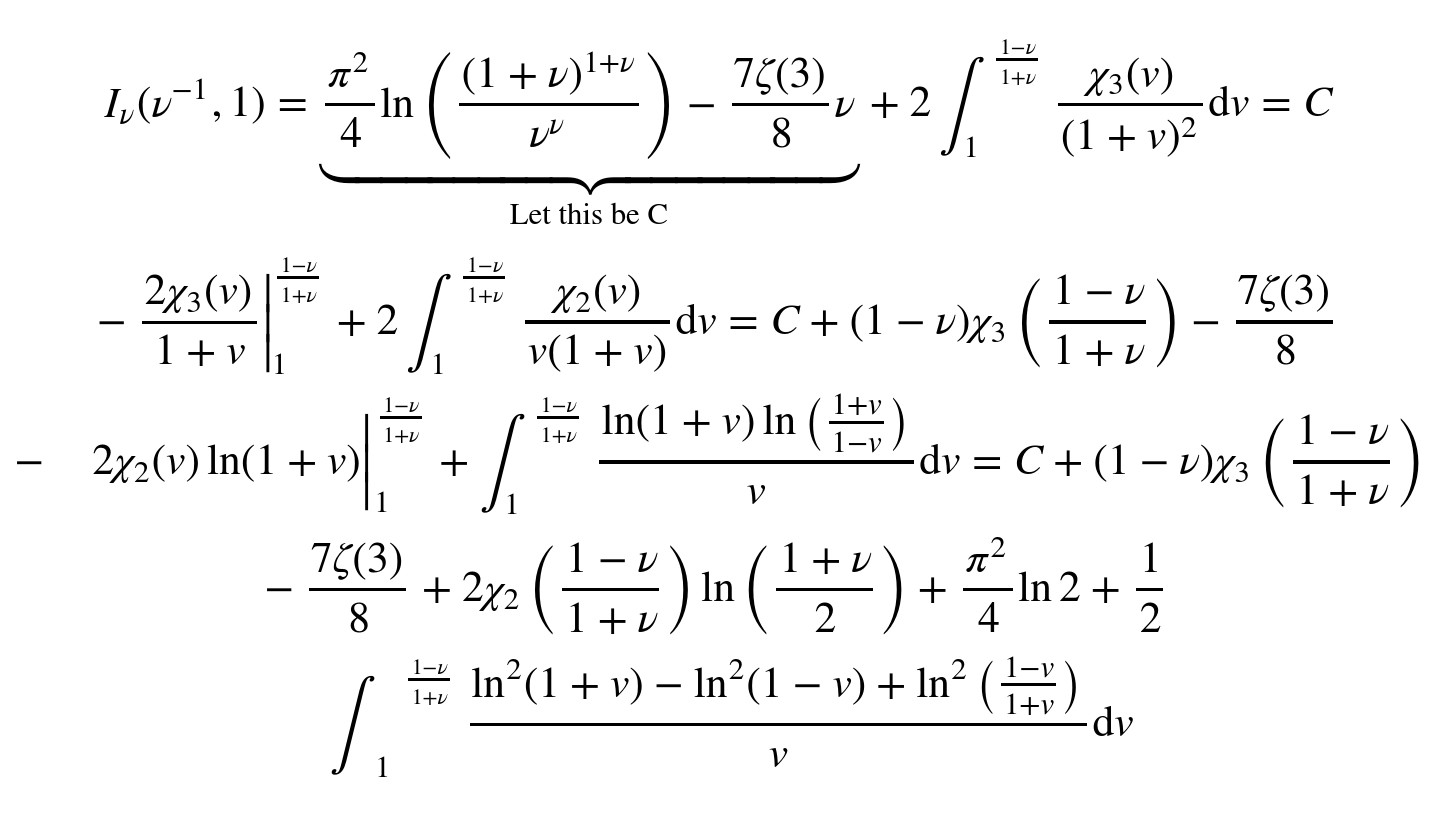
\includegraphics[width=\textwidth]{nolinebreaking}
    \caption{MathJax rendering without enrichment.}
    \label{fig:nolinebreaking}
  \end{minipage}\qquad
  \begin{minipage}{1.05\columnwidth}
    \centering
    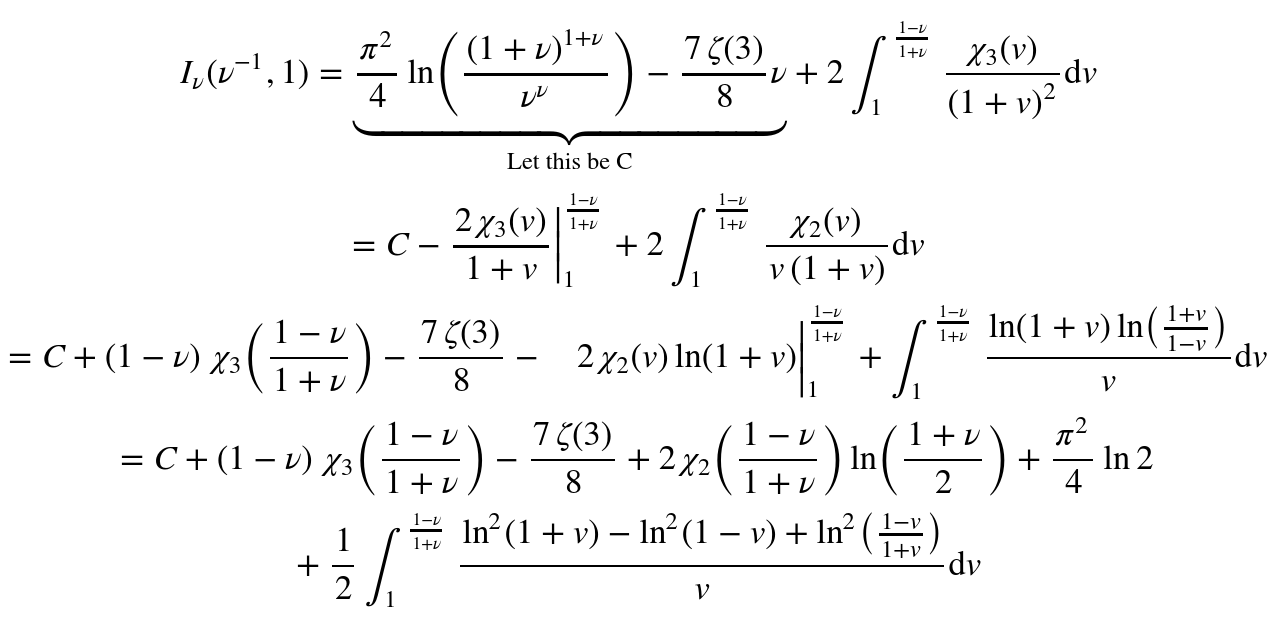
\includegraphics[width=\textwidth]{linebreaking}
    \caption{Rendering of semantically enriched content.}
    \label{fig:linebreaking}
  \end{minipage}
  
\end{figure*}

We demonstrate the effects with an equation found on
%%\href{http://math.stackexchange.com/a/1285149}{math.stackexchange.com}
\url{math.stackexchange.com}, which aligns with our focus on handling arbitrary
content well, not on handling well-prepared content excellently.
Fig.~\ref{fig:nolinebreaking} shows the formula with regular line-breaking,
while Fig.~\ref{fig:linebreaking} has it with semantically
informed line-breaking. Observe that the latter breaks regularly at
equation symbols and does not split individual summands apart.



\section{Semantic Highlighting}
\label{sec:highlighting}

While magnification aims primarily to support readers with low vision, we can
also exploit the semantic features to assist readers with
particular reading difficulties like dyslexia. The choice of high-contrast
colours~\cite{rello2012optimal} and selective
highlighting~\cite{jones2008strategies} can be helpful for reading
comprehension.

Although it is not difficult for MathJax to change colours to high contrast via
CSS styles, this is not necessarily sufficient.  Mathematical expressions are
generally large collections of mostly unconnected symbols in two-dimensional
layout and can therefore be particularly daunting for readers with dyslexia.
Thus it can be beneficial to enable readers to get selective highlighting of
sub-expressions of a complex formula, for example by hovering over parts of an
expression.  While in principle it is possible to use the basic DOM 
structure to identify sub-trees, reading comprehension is enhanced by 
highlighting mathematically meaningful sub-formulas instead.

To illustrate this, consider the first line from Fig.~\ref{fig:linebreaking}.
Highlighting purely on the syntactic
tree, we see that the first level of the MathML tree is effectively a single
row of symbols or combined elements like fractions and sub- or
superscripts. Below we use alternating background colours for the elements
that could be highlighted individually.

\def\cb#1{\colorbox{yellow}{\ensuremath{\!\!#1\!\!}}}
\def\wcb#1{\colorbox{white}{\ensuremath{\!\!#1\!\!}}}
{\footnotesize
\[\cb{I_\nu}
  (
  \cb{\nu^{-1}}
  ,
  \cb{1}
  )
  \cb{=}
  \frac{\pi^2}{4}
  \cb{\ln}
  \left(
    \cb{\frac{(1+\nu)^{1+\nu}}{\nu^\nu}}
  \right)
  \cb{-}
  \frac{7\zeta(3)}{8}
  \cb{\nu}
  +
  \cb{2}
  \int^\frac{1-\nu}{1+\nu}_1
  \cb{\frac{\chi_3(v)}{(1+v)^2}}
  {\rm d}
  \cb{v}
\]
}%
%
Using semantic information, on the other hand, highlighting is done on the
level of the relation and additive operations tree. Consequently we end up with a
much smaller number of sub-expressions and clearer selection of highlighted
sub-formulas.

{\footnotesize
\[\cb{I_\nu(\nu^{-1},1)}
  =\cb{\frac{\pi^2}{4}\ln\left(\frac{(1+\nu)^{1+\nu}}{\nu^\nu}
\right)}-\cb{\frac{7\zeta(3)}{8}\nu}+
\cb{2\int^\frac{1-\nu}{1+\nu}_1\frac{\chi_3(v)}{(1+v)^2}{\rm d}v}
\]
}%
%
In practice, sub-expressions are highlighted when hovering over them with the
mouse pointer, or by switching highlighting on permanently. It also can be
recursively refined for sub-expressions, e.g., hovering on the denominator or
numerator of a fraction only. For permanent highlighting, the 
opaqueness of the background gradually increases in
nested sub-expressions. Nevertheless, in large expressions, highlighting only helps to
some degree to get an overview of the structural composition of a formula; to
aid this further, we introduce a technique for structural abstraction in the next
section.


\section{Structural Abstraction}
\label{sec:abstraction}

Users with reading challenges, such as dylexia, can quickly become 
overhelmed by the complex two-dimensional layout of mathematical 
expressions. Such readers can be assisted by simplifying the structure of
the formula initially and letting them individually explore the equation by
manually expanding selected sub-expressions.

We have implemented this via a user interface using MathML's \texttt{maction}
element (cf.~\cite[3.7.1]{MathML3}). It allows users to explore the content using
click, keyboard, and touch events. \texttt{maction} elements are nested so
that only the next level of the collapse is revealed.
The element indicating collapsed content is a simple Unicode
construction, \collapse{X}, with X indicating the top-level structure that was
collapsed. For example we use \collapse{+} to indicate a sum,
\collapse{\mathrm{\int}} for an integral, etc.

\begin{figure*}[t]
  \begin{minipage}{.08\textwidth}
    \centering
    $\collapse{=...}$
  \end{minipage}\qquad\qquad
  \begin{minipage}{.1\textwidth}
    \begin{align*}
      \collapse{\mathrm{f}()} & = \collapse{+} \\
                              & = \collapse{+} \\ 
                              & = \collapse{+} \\ 
                              & = \collapse{+} + \collapse{\cdot} + \collapse{\cdot} \\
                              & \collapse{...} 
    \end{align*}
  \end{minipage}
  \begin{minipage}{.25\textwidth}
    \centering
    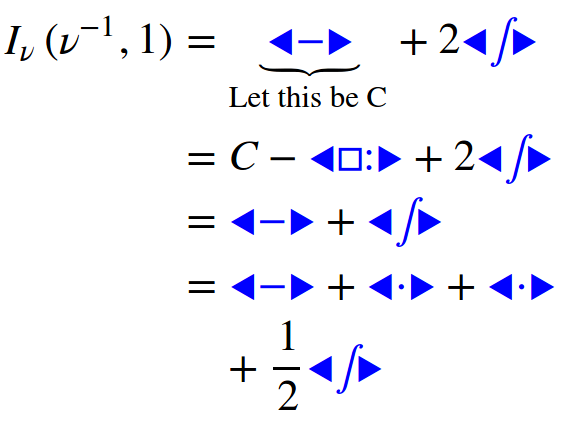
\includegraphics[width=\textwidth]{expand1}
  \end{minipage}\qquad\quad
  \begin{minipage}{.25\textwidth}
    \centering
    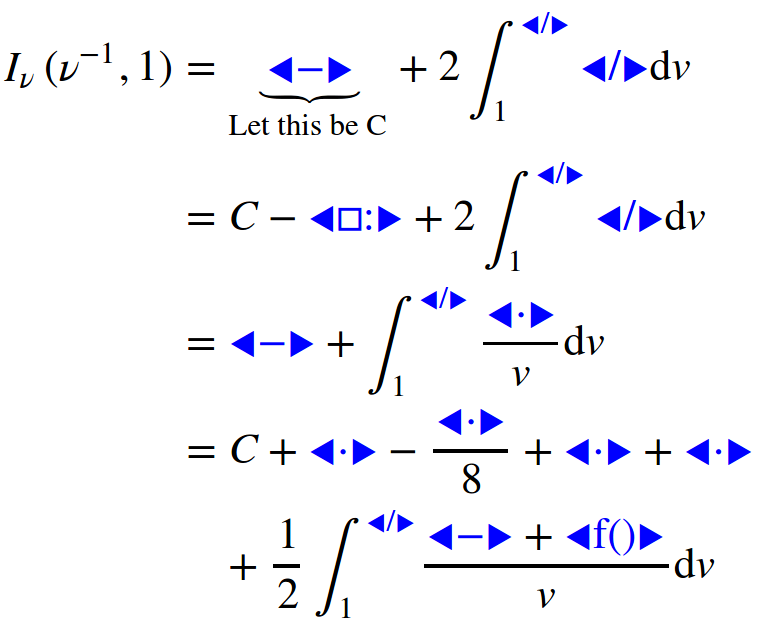
\includegraphics[width=\textwidth]{expand2}
  \end{minipage}
  \caption{Four different stats of Collapse of example equation.}
  \label{fig:collapse}
\end{figure*}


Fig.~\ref{fig:collapse} demonstrates four different states of collapse of our
example equation.  To determine which parts are collapsed, our algorithm
somewhat surprisingly does not calculate sub-expression width since these are
not available before rendering. Instead, it estimates the complexity of an
expression by recursively evaluating the enriched MathML tree. For example,
token elements are assigned a complexity value according to their string content
while more complex elements such as roots or fractions are assigned the sum of
their children's complexity measures modified by a value corresponding to their
own visual complexity. Cut-off values for each semantic type are then used to
decide which expressions are collapsed. The parameters (character weight,
operator modifier, cut-off) are configurable by the content author.

\section{Aural Rendering}

In a final step, we now exploit our semantic enrichment, and in particular the
structural abstraction, as an accessibility service for screen readers.  Currently,
MathJax already provides support for third-party screen readers by embedding the
MathML representation for formulas as hidden elements into the DOM. This can be
picked up by a screen reader to either voice directly (e.g., in the case of
ChromeVox or VoiceOver), or by using a third-party library like
MathPlayer~\cite{soiffer2005mathplayer} for speech translation. Thus users still
have to depend on their screen reader's ability to understand MathML to provide either of these two
capabilities.  Despite being a pragmatic solution today, this severely
limits accessibility as it disconnects visual and AT rendering completely.

In order to make users independent of a screen reader's Math capabilities,
MathJax now exploits direct access to the speech-rule engine~\cite{Sorge14}
that generates the semantic-tree transformation in the first place and provides
aural renderings of mathematical expressions that can be directly exposed to a
screen reader.  This feature is offered together with an interface for
interactive exploration of the mathematical expression either along the
syntactic structure or the semantic tree.

The real novelty in exploiting the semantic enrichment, however, is that it
enables us to not only display but also voice semantically informed summaries of
mathematical expressions using appropriate speech rules. This way, even complex
formulas can be described in a concise manner, aiding a casual reading
experience. The idea is that the reader gets an impression of what type of formula
is there while reading, and can then choose to get more information or dive
deeper into parts of the formula should they so desire.

The basic principle is to exploit the structure provided by the
collapse/expansion mechanism implemented via the \texttt{maction}
elements. Speech rules then can directly interpret the top level of the
collapsed expression, effectively voicing only the summary symbol together with
the rest of the equation. Alternatively, slightly more expressive speech rules
can voice a summary of the underlying collapsed expression.

For example, in the case of the quadratic formula, the only collapse possible is
the sum on the left-hand side of the equation. Two alternative ways of speaking
it are ``Sum equals~0'' or ``Sum with three summands equals 0.''

This feature can be integrated into the expansion interface by providing
standard cursor key bindings to expand step-by-step the collapsed parts
of an expression while speaking the newly revealed sub-formulas.  Technically, we
achieve this by introducing a dedicated assertive ARIA live region into the DOM
and updating it with the desired speech output. Speech strings for a formula and
all its sub-expressions can be pre-computed and embedded
into the MathML along-side the semantic information as an additional data
attribute, thereby exposing it also in the rendered DOM elements. This allows us
to simply retrieve the string and update the ARIA live region, allowing
its content to be voiced by most screen readers.

Fig.~\ref{fig:embedded-speech} depicts the enriched MathML expression with
embedded speech strings for the quadratic formula. Note the summary
message in the \texttt{maction} element. By default we currently employ the
MathSpeak rule set~\cite{MathSpeak} for embedded speech generation, with the
exception of the summarising, where we have a small, newly developed
set. This can be changed to other rule sets, e.g., the
original ChromeVox rules.

The advantage of directly embedding speech is that it is available without lag
when voicing the expression. However, speech strings are always generated, even
in the case when no screen reader is present, which can become computationally
expensive on pages with many mathematical expressions. In addition, it is more
difficult to customise speech rules programmatically on pages for specialised
mathematical content.

To avoid computational overhead and support easier customisation, an alternative
is to generate speech strings on the fly, if and when necessary, and expose them
via the ARIA live region. While this has the advantage that it is easy to
customise rules or use different rule sets altogether --- and we indeed provide
a simple API that allows for adding or modifying speech rules --- the recursive
nature of generating speech rules can lead to computational overhead, in
particular when exploring sub-expressions step-wise. As a consequence, we have
implemented a caching mechanism that avoids multiple speech generations for the
same sub-expressions.

\begin{figure}[t] 
\lstxml
{\begin{lstlisting}[language=html]
<math speech="sum with three summands equals 0" complexity="7">
  <maction complexity="2" speech="sum with three summands">
    <mtext mathcolor="blue">&#x25C2;+&#x25B8;</mtext>
    <mrow speech="a x squared plus b x plus c" complexity="24.8">
      <mrow speech="a x squared" complexity="10.8">
        <mi speech="a" complexity="1">a</mi>
        <mo speech="times" complexity="1">&#x2062;</mo>
        <msup speech="x squared" complexity="5.8">
          <mi speech="x" complexity="1">x</mi>
          <mn speech="2" complexity="1">2</mn>
        </msup>
      </mrow>
      <mo speech="plus" complexity="1">+</mo>
      <mrow speech="b x" complexity="6">
        <mi speech="b" complexity="1">b</mi>
        <mo speech="times" complexity="1">&#x2062;</mo>
        <mi speech="x" complexity="1">x</mi>
      </mrow>
      <mo speech="plus" complexity="1">+</mo>
      <mi speech="c" complexity="1">c</mi>
    </mrow>
  </maction>
  <mo speech="equals" complexity="1">=</mo>
  <mn speech="0" complexity="1">0</mn>
</math>
\end{lstlisting}}
\caption{Embedded speech strings and complexity for the quadratic
  formula. Observe that other semantic attributes have been omitted.}
\label{fig:embedded-speech}
\end{figure}


\section{Conclusions}
\label{sec:conc}

We have presented the advanced accessibility features of MathJax that are
based on a new semantic enrichment procedure for Presentation MathML. In
particular, the novel approach to responsive rendering of equations shows promise
for more advanced AT techniques.  Although we have not yet had the opportunity
to do extensive user testing, since our code is developed publicly on our GitHub
repository, we have already had some user feedback. Initial reactions have been
extremely positive, but we hope to pursue collaborations for wider, real-world
testing in 2016.

While the presented AT extensions are not yet available in core MathJax, we plan
to release a MathJax extension usable with current MathJax versions and to move
the advances closer to the core during our upcoming work on MathJax v3.0.
As our tools can run both client- and server-side (via NodeJS), they can
be leveraged both by page authors and by end users (via bookmarklets or
browser extensions), as well as directly in assistive technology.

We believe our work can be greatly expanded. First, the heuristics can be
augmented to enhance precision of the analysis. Second, subject-specific rules
can be implemented to improve precision; in the long term, this could enable the
combination of natural-language processing tools to augment our heuristics by
analysing the surrounding context. Third, we believe the semantic enrichment of
MathML can inform web standards development regarding improvements to MathML and
ARIA to enable other AT solutions to build on our results.

\subsection*{Acknowledgement}
\noindent The work was supported by the Alfred P. Sloan Foundation.

\bibliographystyle{IEEEtran}
% \bibliography{ads16}
% Generated by IEEEtran.bst, version: 1.12 (2007/01/11)
\begin{thebibliography}{10}
\providecommand{\url}[1]{#1}
\csname url@samestyle\endcsname
\providecommand{\newblock}{\relax}
\providecommand{\bibinfo}[2]{#2}
\providecommand{\BIBentrySTDinterwordspacing}{\spaceskip=0pt\relax}
\providecommand{\BIBentryALTinterwordstretchfactor}{4}
\providecommand{\BIBentryALTinterwordspacing}{\spaceskip=\fontdimen2\font plus
\BIBentryALTinterwordstretchfactor\fontdimen3\font minus
  \fontdimen4\font\relax}
\providecommand{\BIBforeignlanguage}[2]{{%
\expandafter\ifx\csname l@#1\endcsname\relax
\typeout{** WARNING: IEEEtran.bst: No hyphenation pattern has been}%
\typeout{** loaded for the language `#1'. Using the pattern for}%
\typeout{** the default language instead.}%
\else
\language=\csname l@#1\endcsname
\fi
#2}}
\providecommand{\BIBdecl}{\relax}
\BIBdecl

\bibitem{karshmer2007mathematics}
A.~Karshmer, G.~Gupta, and E.~Pontelli, ``Mathematics and accessibility: a
  survey,'' in \emph{Proc. 9th ICCHP}, vol. 3118, 2007, pp. 664--669.

\bibitem{soiffer2005mathplayer}
N.~Soiffer, ``Mathplayer: web-based math accessibility,'' in \emph{Proceedings
  of the 7th international ACM SIGACCESS conference on Computers and
  accessibility}.\hskip 1em plus 0.5em minus 0.4em\relax ACM, 2005, pp.
  204--205.

\bibitem{MathML3}
D.~Carlisle, P.~Ion, and R.~Miner, ``{MathML} version 3.0,'' W3C Recommendation,
  2010, \url{www.w3.org/TR/MathML3}.

\bibitem{HTML5}
  Wide Web Consortium, ``HTML version 5.0,'' World
  W3C Candidate Recommendation, 2013, available at
  \url{www.w3.org/TR/html5}.

\bibitem{MathJax2.5}
M.~Consortium, ``{MathJax} version 2.5,'' 2014, \url{www.mathjax.org}.

\bibitem{Sorge14}
V.~Sorge, C.~Chen, T.~Raman, and D.~Tseng, ``Towards making mathematics a first
  class citizen in general screen readers,'' \emph{W4A 2014}. ACM.

\bibitem{voiceover}
``Apple voiceover,'' \url{https://www.apple.com/accessibility/osx/voiceover/}.

\bibitem{MathSpeak}
A.~Nemeth, ``Mathspeak,'' www.gh-mathspeak.com/, 2005.

\bibitem{Maple}
Maplesoft, ``Documentation Center: MathML package,'' 2012.
  \url{http://www.maplesoft.com/support/help/Maple/view.aspx?path=MathML}.

\bibitem{Mathematica}
{Wolfram Language}, ``Working with {MathML},'' 2012,
  \url{http://reference.wolfram.com/mathematica/XML/tutorial/MathML.html}.

\bibitem{miller2010latexml} B.~Miller, ``LateXML: A LaTeX to XML converter,'' 2010.
\url{http://dlmf.nist.gov/LaTeXML}

\bibitem{mooresemantic}
\BIBentryALTinterwordspacing
R.~Moore, ``{Semantic enrichment of mathematics via
  `tooltips'},'' in \emph{Proc. of CICM 2015}, LNCS 9150, Springer, 2015.
\BIBentrySTDinterwordspacing

\bibitem{SnuggleTeX}
D.~McKain, ``Snuggletex v1.2.2,'' University of Edinburgh, 2010,
  \url{http://www2.ph.ed.ac.uk/snuggletex/}

\bibitem{web1}
\url{www.smashingmagazine.com/2013/07/08/choosing-a-responsive-image-solution/}.

\bibitem{smashSvg}
\url{www.smashingmagazine.com/2014/03/05/rethinking-responsive-svg/}.

\bibitem{zurbTable}
\url{zurb.com/playground/projects/responsive-tables/index.html}.

\bibitem{rello2012optimal}
L.~Rello and R.~Baeza-Yates, ``Optimal colors to improve readability for people
  with dyslexia,'' in \emph{Text Customization for Readability}, 2012.

\bibitem{jones2008strategies}
R.~Jones, ``Strategies for reading comprehension: Selective underlining,''
  2008.
\bibitem{browser_stats}
``Usage share of web browsers,'' \url{https://en.wikipedia.org/wiki/Usage_share_of_web_browsers#Summary_tables}.
\end{thebibliography}


\end{document}


%%% Local Variables:
%%% mode: latex
%%% TeX-master: t
%%% End:
